\documentclass[]{book}
\usepackage{lmodern}
\usepackage{amssymb,amsmath}
\usepackage{ifxetex,ifluatex}
\usepackage{fixltx2e} % provides \textsubscript
\ifnum 0\ifxetex 1\fi\ifluatex 1\fi=0 % if pdftex
  \usepackage[T1]{fontenc}
  \usepackage[utf8]{inputenc}
\else % if luatex or xelatex
  \ifxetex
    \usepackage{mathspec}
  \else
    \usepackage{fontspec}
  \fi
  \defaultfontfeatures{Ligatures=TeX,Scale=MatchLowercase}
\fi
% use upquote if available, for straight quotes in verbatim environments
\IfFileExists{upquote.sty}{\usepackage{upquote}}{}
% use microtype if available
\IfFileExists{microtype.sty}{%
\usepackage{microtype}
\UseMicrotypeSet[protrusion]{basicmath} % disable protrusion for tt fonts
}{}
\usepackage[margin=1in]{geometry}
\usepackage{hyperref}
\hypersetup{unicode=true,
            pdftitle={Sleep quality analysis},
            pdfauthor={Arturo Laflor},
            pdfborder={0 0 0},
            breaklinks=true}
\urlstyle{same}  % don't use monospace font for urls
\usepackage{natbib}
\bibliographystyle{apalike}
\usepackage{longtable,booktabs}
\usepackage{graphicx,grffile}
\makeatletter
\def\maxwidth{\ifdim\Gin@nat@width>\linewidth\linewidth\else\Gin@nat@width\fi}
\def\maxheight{\ifdim\Gin@nat@height>\textheight\textheight\else\Gin@nat@height\fi}
\makeatother
% Scale images if necessary, so that they will not overflow the page
% margins by default, and it is still possible to overwrite the defaults
% using explicit options in \includegraphics[width, height, ...]{}
\setkeys{Gin}{width=\maxwidth,height=\maxheight,keepaspectratio}
\IfFileExists{parskip.sty}{%
\usepackage{parskip}
}{% else
\setlength{\parindent}{0pt}
\setlength{\parskip}{6pt plus 2pt minus 1pt}
}
\setlength{\emergencystretch}{3em}  % prevent overfull lines
\providecommand{\tightlist}{%
  \setlength{\itemsep}{0pt}\setlength{\parskip}{0pt}}
\setcounter{secnumdepth}{5}
% Redefines (sub)paragraphs to behave more like sections
\ifx\paragraph\undefined\else
\let\oldparagraph\paragraph
\renewcommand{\paragraph}[1]{\oldparagraph{#1}\mbox{}}
\fi
\ifx\subparagraph\undefined\else
\let\oldsubparagraph\subparagraph
\renewcommand{\subparagraph}[1]{\oldsubparagraph{#1}\mbox{}}
\fi

%%% Use protect on footnotes to avoid problems with footnotes in titles
\let\rmarkdownfootnote\footnote%
\def\footnote{\protect\rmarkdownfootnote}

%%% Change title format to be more compact
\usepackage{titling}

% Create subtitle command for use in maketitle
\newcommand{\subtitle}[1]{
  \posttitle{
    \begin{center}\large#1\end{center}
    }
}

\setlength{\droptitle}{-2em}
  \title{Sleep quality analysis}
  \pretitle{\vspace{\droptitle}\centering\huge}
  \posttitle{\par}
  \author{Arturo Laflor}
  \preauthor{\centering\large\emph}
  \postauthor{\par}
  \predate{\centering\large\emph}
  \postdate{\par}
  \date{2017-04-28}

\usepackage{booktabs}
\usepackage{amsthm}
\usepackage{multirow}
\usepackage{multicol}
\usepackage{float}
\usepackage{tabularx}
\makeatletter
\def\thm@space@setup{%
  \thm@preskip=8pt plus 2pt minus 4pt
  \thm@postskip=\thm@preskip
}
\makeatother

\begin{document}
\maketitle

{
\setcounter{tocdepth}{1}
\tableofcontents
}
\chapter{Prerequisites}\label{prerequisites}

\chapter{Introduction}\label{intro}

\hypertarget{data-adquisition}{\chapter{\texorpdfstring{\protect\hyperlink{data-adquisition}{Data
adquisition}}{Data adquisition}}\label{data-adquisition}}

\chapter{\texorpdfstring{\protect\hyperlink{data-preprocess}{Data
pre-process}}{Data pre-process}}\label{data-pre-process}

\hypertarget{feature-selection}{\chapter{\texorpdfstring{\protect\hyperlink{feature-selection}{Feature
selection}}{Feature selection}}\label{feature-selection}}

This section describes the process that we perform to reduce the
dimension of the sleep hygiene data set that contains the features to
model the quality of sleep for respondents of the survey described in
chapter \ref{data-adquisition}. There exist two ways to addressed
dimensionality reduction, feature extraction and feature selection.
Feature extraction, consists in generate a new and small feature space.
The application of a technique of feature extraction produce new
features based in original ones. The new dataset is not understandable
in terms of the original dataset, rather, it is an abstraction of this
and its visualization have no practical meaning. On the other hand,
feature selection as ilustrate the Fig.
\ref{fig:feature-selection-process} choose a small subset of the
relevant features from the original dataset according to certain
relevance evaluation criterion, which usually leads to better learning
performance, lower computational cost, and better model interpretability
\citep{Tang2014}.

\begin{figure}[H]

{\centering 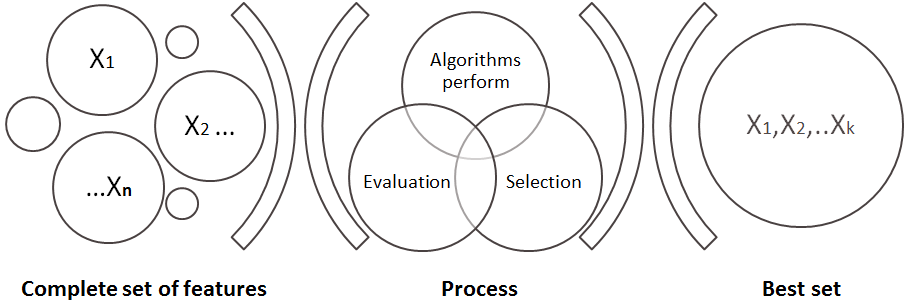
\includegraphics[width=0.8\linewidth]{images/feature-selection-process} 

}

\caption{Feature selection Process}\label{fig:feature-selection-process}
\end{figure}

For the purposes of this study, the technique of selection of
characteristics is the most appropriate. Our interest in reducing
dimensionality is not related to the decrease in computational cost,
rather, the purpose is to decrease the number of predictive variables
due to the high cost of design and infrastructure that means capturing
21 different signals through sensors. If it is possible to characterize
a high percentage of the phenomenon, through a reduced number of factors
of sleep hygiene, the design of the system will be more feasible and
less expensive.

The model accuracy for prediction of the sleep quality with the subset
of features must be better than the training model using the total of
sleep hygiene features.

\section{\texorpdfstring{\protect\hyperlink{feature-selection-model}{Feature
selection
models}}{Feature selection models}}\label{feature-selection-models}

In 1996, \citep{Liu1998} proposes two models to achieve the reduction of
features, that have been used as basis of diverse algorithms still in
force. The filter model (see Figure \ref{fig:filter-model}) that uses as
criterion of feature selection, some attributes concerning only to the
data domain. Especifiacally in this model, Liu et. al. proposes that it
is posible to analyze and make decisions over irrelevance or relevance
of features based in measure information gain, dependence, distance and
consistency.

\begin{figure}[H]

{\centering 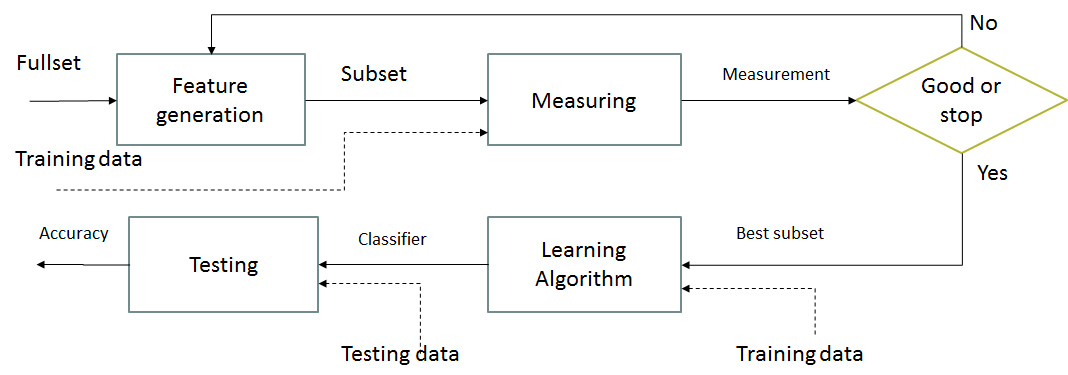
\includegraphics[width=0.6\linewidth]{images/filter-model} 

}

\caption{Filter model proposed by Liu et. al.}\label{fig:filter-model}
\end{figure}

The second model showed in Fig. \ref{fig:wrapper-model} proposed is the
wrapper model that uses the accuracy of prediction as selection
criterion, it means that this techniques are committed with a particular
classifier in this stage of the learning process.

\begin{figure}[H]

{\centering 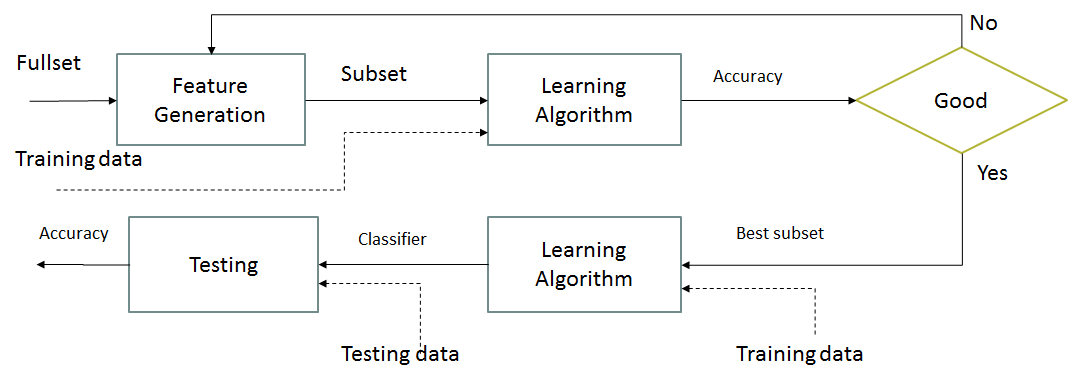
\includegraphics[width=0.6\linewidth]{images/wrapper-model} 

}

\caption{Wrapper model proposed by Liu et. al.}\label{fig:wrapper-model}
\end{figure}

Both models have advanteges and disadvantages, techniques based in
filter model, performs better than others based in wrapper model,
however, researchers have no idea over prediction accuracy during the
feature selection process. Some practitioners don't preffer to use these
techniques because if accuracy prediction is not achieved in the
proposed level, the first steep can be regarded as a waste of time. On
the other hand, some researchers argued that select features based in
determinated classifier, reduces the possibility to use other classifier
to generate the prediction model, in this sense, the classifier to
generate the final model should be choosed at the begining, and it is
not convenient for all problems. In these order of thinks,
\citep{Kelleher2015} comment that wrapper models are more
computationally expensive than filters models and that the argument of
they are uncertain models respect to the accuracy, is not at all valid
since filters model often generate models with good accuracy.

Additionaly, \citep{Liu1998} highlight \emph{Search}, \emph{Scheme} and
\emph{measure} as three important concepts that help to decide what
technique is the most appropriate for an specific problem of
dimentionality reduction by feature selection (see Fig.
\ref{fig:main-dimensions-dr}). Search refers to the activity of choose
features in non deterministic, heuristic or complete form, Scheme must
be determine if the search will be forward, backward or in random mode,
and, measure has to do with tree ways to establish the threshold for
stopping the feature search, the criterion used are accuracy,
consistency, and, classic criterion involving distance, information gain
and dependence.

\begin{figure}[H]

{\centering 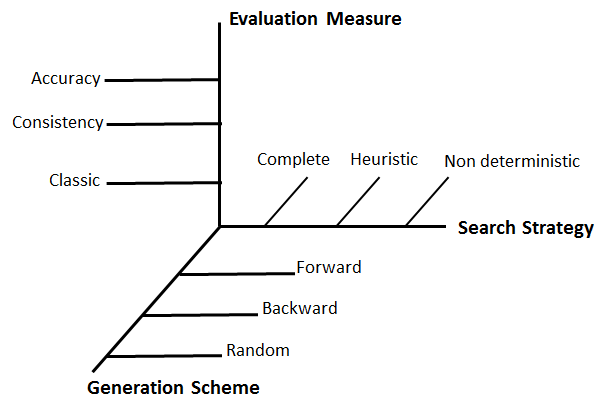
\includegraphics[width=0.6\linewidth]{images/main-dimensions-in-feature-selection} 

}

\caption{Main dimensions in feature selection, Liu et. al.}\label{fig:main-dimensions-dr}
\end{figure}

A third type of model has been proposed in last years, these models are
called \textbf{embedded models}, since they allow practitoners select
features while the prediction model is built. Embedded models have the
advantage of filters model in terms of low computational cost, and take
the advantage of wrapper model, because the prediction accuracy and
classification model are involved in the process. \citep{Tang2014}
describe three type of embedded methods as we shows in the Table
\ref{tab:table-embedded-methods}.

\begin{table}[h]
\centering
\caption{Embedded methods as \cite{Tang2014} describes and quoted verbatim in his paper.}
\label{tab:table-embedded-methods}
\begin{tabular}{|>{\centering\arraybackslash}p{3cm}|>{\arraybackslash}p{10cm}|>{\centering\arraybackslash}p{2cm}|}
\hline Method & Description & Cite \\ 
\hline Pruning & Utilizing all features to train a model and then attemp to eliminate some features by setting the corresponding coefficients to 0, while maintaining model performance such as recursive feature elimination using support vector machines (SVM) & \cite{Guyon2002} \\ 
\hline Build-in & Mechanism for feature selection as ID3 and C4.5 & \cite{Quinlan1986,Quinlan1993} \\ 
\hline Regularization & Utilices objective functions that minimize fitting errors and in the mean time force the coefficients to be small or ti be exact zero. & \cite{Ma2008} \\ 
\hline 
\end{tabular} 
\end{table}

These models are representative of the theoretical basis where a lot of
algorithms for selection features in last twenty years have been fueled.
Likewise four concepts are the most important and have been used for the
generation of different feature selection algorithms in last two
decades: distance, accuracy, inconsistency and information gain.

\begin{itemize}
\tightlist
\item
  Distance: The main goal to use distance, is to find similarity among
  instances in a dataset. The Equation proposed by Minkowski (see eq.
  \eqref{eq:Minkowski}) is a generalization of the distances that are used
  in MLA. The most common distances are the particular cases where
  \(p=1\) called Manhatan distance (see Eq. \eqref{eq:Manhattan}) and
  where \(p=2\), the well known Euclidian distance (see Eq.
  \eqref{eq:Euclidean}). (All three equations were taken from
  \citep{Kelleher2015}). The implication of use different values of
  \(p\) will be noted in the difference between two values of any
  feature in the final distance, it is directly proportional to the
  value of \(p\). It means that large differences between two features
  in an instance, impact stronger in the final result when \(p\) grows.
\end{itemize}

\begin{equation}
      Euclidean(A,B)=\sqrt{(a_1-b_1)^2+(a_2-b_1)^2+\dots+(a_n-b_n)^2}
      \label{eq:Euclidean}
\end{equation}

\begin{equation}
      Manhattan(a,b)=\sum_{i=1}^{m}abs(a[i]-b[i])
      \label{eq:Manhattan}
\end{equation}

\begin{equation}
    Minkowski(a,b)=\left({\sum_{i=1}^{m}abs(a[i]-b[i])^p}\right)^{\frac{1}{p}}
    \label{eq:Minkowski}
\end{equation}

\begin{itemize}
\tightlist
\item
  Accuracy: Accuracy refers to the successes that a model had to predict
  each instance of a dataset, it is opposed to the miscalssification
  error as \citep{Kelleher2015} defines in
  \eqref{eq:math-misclassification-rate} and \eqref{eq:math-accuracy}
  equations. These two equation take relevance when accuracy is analized
  in the context of confusion matrix, a tool widely used to report the
  outcomes of the prediction thorugh a model. The confusion matrix
  together with the Receiver Operating Characteristics (ROC) curve,
  provides understanding and visualization of the specificity and
  sensibility, the most important metrics for evaluations of the models,
  especially in the health context.
\end{itemize}

\begin{equation}
  misclassification\ rate=\frac{(FP+FN)}{(TP+TN+FP+FN)}
  \label{eq:math-misclassification-rate}
\end{equation}

\begin{equation}
  accuracy=\frac{(TP+TN)}{(TP+TN+FP+FN)}
  \label{eq:math-accuracy}
\end{equation}

\begin{itemize}
\item
  Inconsistency: An inconsistency refers that two instances have the
  same value in all descriptive features, but they belong to a different
  class. We can compute two values to measure the inconsistency for a
  subset of features in a dataset. The first value, which is called the
  inconsistency count (\(IC\)), can be defined as \(IC=nM-LCI\), where
  \(nM\) is the number of instances that coincide in all descriptive
  features, and, \(LCI\) is the largest class of the clases that are
  involved in this particular group of instances. The second value, is
  the inconsistency rate defined as \(IR=\frac{\sum_{i=0}^{m}IC_i}{N}\),
  where \(m\) is the total of groups of matching instances in the
  dataset.
\item
  Information Gain: Is a measure of the relevance that a predictive
  variable offers in relation to the target variable. To understand the
  concept of information gain, it is necessary to first understand the
  concept of information entropy as was raised by Shannon in 1948. In a
  dataset, an entropy value represents the heterogenity/homogenity of
  the target variable, in others words, if we have large probability of
  success to predict an outcome in the target feature, we have a set
  with small entropy and viceversa.
\end{itemize}

The process to calculate the information gain of one feature can be
sumarized as follows:

\begin{enumerate}
\def\labelenumi{\arabic{enumi}.}
\tightlist
\item
  Compute the total entropy.
\item
  Split the target feature in the levels of the predictive feature.
\item
  Compute the entropy of the target variable in each subset generate,
  and multiply the result by its weight. The weight is computed by
  dividing the number of instances in the subset, among the total number
  of instances in the dataset.
\item
  Subtrac form the total entropy, the entropy computed in the steps
  \(2\) y \(3\).
\item
  Sort the results in descending order to identify which are the best
  and the worst features in terms of provide information to characterize
  the phenomenon.
\end{enumerate}

\section{Feature selection process}\label{feature-selection-process}

Five methods for feature selection were selected to make the process of
selection the relevant sleep hygiene factors. Each method works with the
complete set of features and the total of the data, after the process,
the features were ordered by relevance in descending order in each
method. A merge process was performed to choose those features that were
ranked in the first places in each method. This process ensure that
features choosen are relevant features because the theory and math
behind the methods are different in each one. The Fig.
\ref{fig:four-methods-of-feature-selection} shows four of the six
methods (for space reasons), and the corresponding features (Factor) and
weights (Pesos) in descending order. The Fig. \ref{fig:selected-factors}
shows the outcomes of selected factors by the merge process. The left
side, is the table with features and the corresponding weights in the
best algorithms, in these case Random Forest (RF), Logistic Regression
(LR) and Logistic Regression with Cross Validation (LR\_CV). The right
side ilustrate in a line-graph, the comparisson of the data in the table
of the left side. Both figures are screens capture of the application
developed on Shiny R-Studio for this specific purpose.

\begin{figure}[H]

{\centering 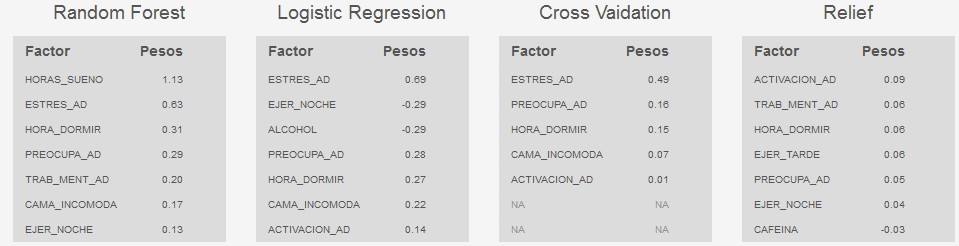
\includegraphics[width=0.8\linewidth]{images/four-methods-of-feature-selection} 

}

\caption{Results of four methods after performs Feature Selection}\label{fig:four-methods-of-feature-selection}
\end{figure}

\begin{figure}[H]

{\centering 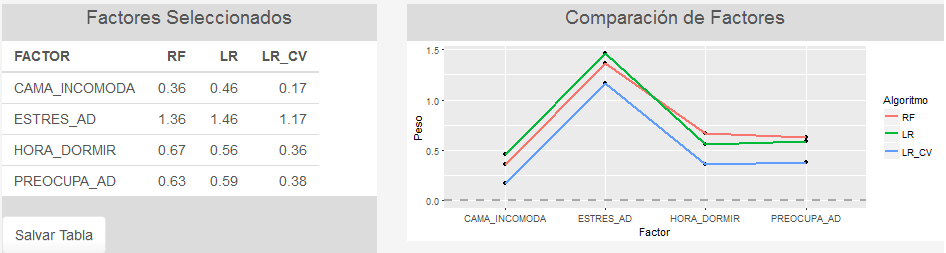
\includegraphics[width=0.8\linewidth]{images/selected-factors} 

}

\caption{Outcomes for selected factors after the merge process}\label{fig:selected-factors}
\end{figure}

From the original 21 hygiene factors that in theory are the predictive
variables to characterize the sleep quality, the feature selection
algorithms choose four features. It means that the remaining seventeen
features, there are not relevant factors to characterize the phenomenon
on this population. As additional information related with the studied
phenomenon, it is possible to note that two features closely related
with the state of mind, are present among features selected. Even, one
of this two features, the stress before go to the bed (ESTRES\_AD), is
the most relevant feature of the four selected. If this selection
provides the best model to characterize the phenomenon, a great
challenge is perceived in the near future, due to how difficult it can
be to measure a subjective variable, by means of an electronic device.

\chapter{Methods}\label{methods}

\chapter{Applications}\label{applications}

\chapter{Placeholder}\label{placeholder}

\chapter{Final Words}\label{final-words}

\bibliography{packages,book}


\end{document}
